\section{Fog Computing-Based Architectures}
\label{sec:3}

%-----------------------------------------------------------------subsection1

\subsection{Architecture}

The architecture explains how fog computing extends services offered by the cloud i.e., computation, communication, and storage to the edge of the network \cite{mukherjee2018survey}.

%------------------------------subsubsection1.1

\subsubsection{Three-tier architecture}

Fig. \ref{fig:three-tier fog computing architecture} shows the three-tier architecture which is broadly used among all the architectures of fog computing \cite{mukherjee2018survey}. \par

The bottom tier consists of end devices such as IoT devices, sensor nodes, smart devices, and so on. These end devices are also known as Terminal Nodes (TNs) \cite{mukherjee2018survey}. These nodes can sense and capture the data \cite{webpage} and are equipped with Global Positioning System (GPS) \cite{mukherjee2018survey}. TNs are heterogeneous that work irrespective of technology, communication mode, hardware, and OS \cite{webpage}. \par

\begin{figure}[H]
    \centering
    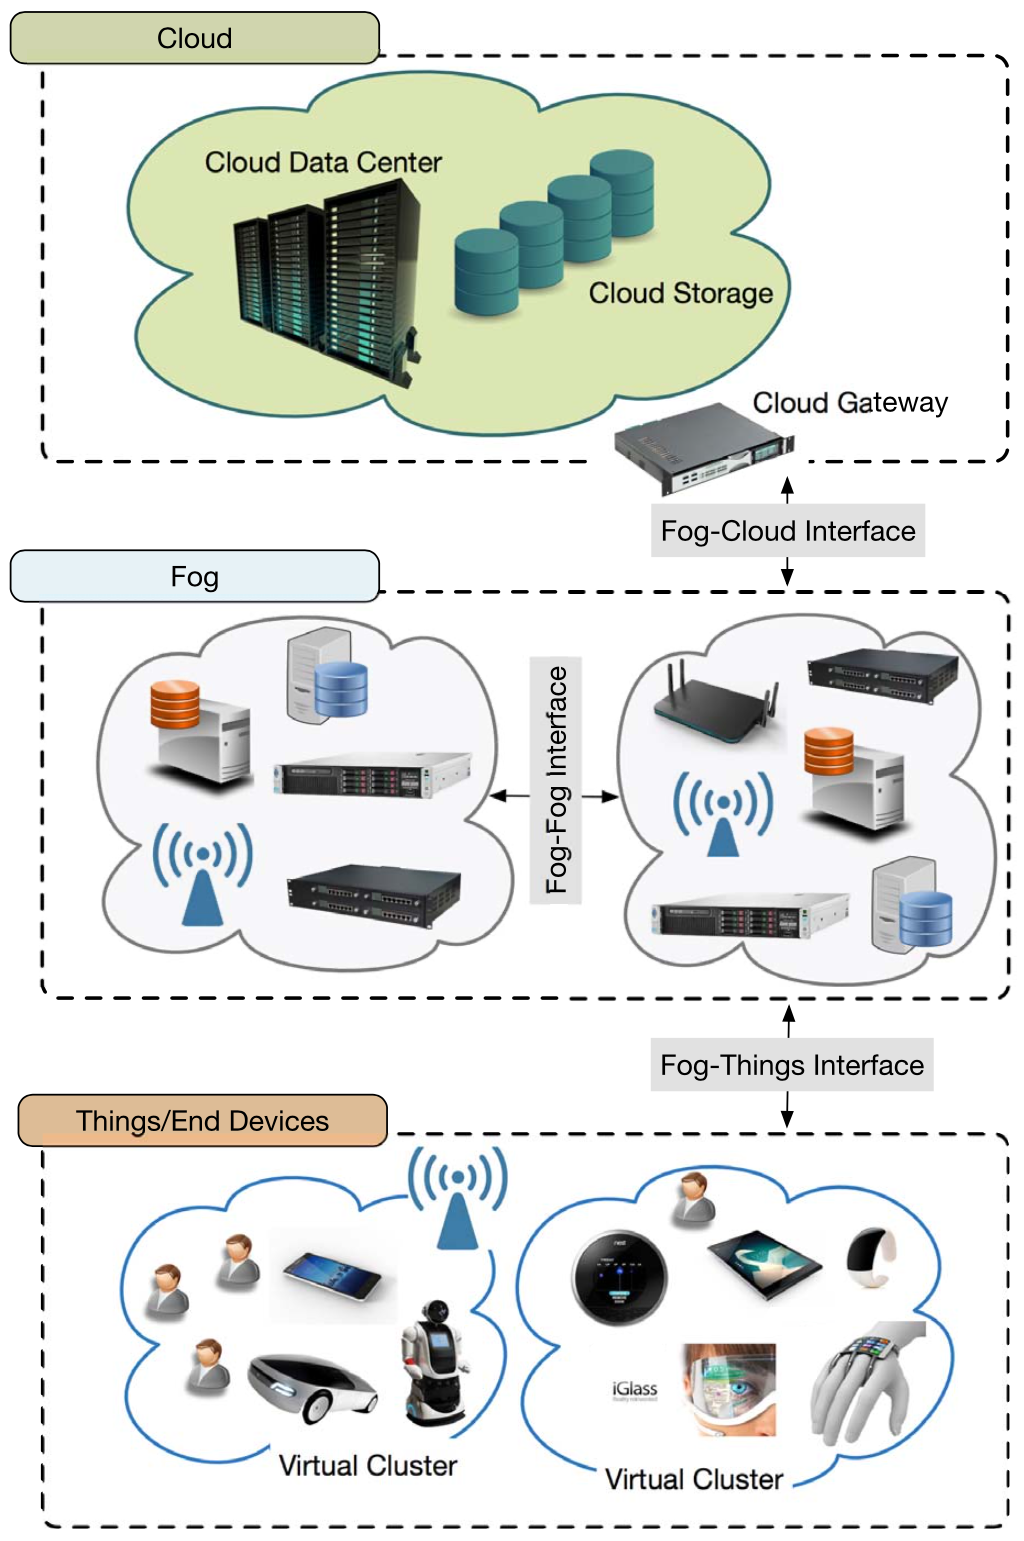
\includegraphics[width=.5\linewidth]{image/Three-tier fog computing architecture.png}
    \caption{Three-tier fog computing architecture}
    \caption*{img src: \cite{mukherjee2018survey}}
    \label{fig:three-tier fog computing architecture}
\end{figure}

The fog tier is known as the fog computing layer which consists of network devices like routers, gateways, switches, Access Points (APs), base stations, fog servers, and so on \cite{mukherjee2018survey}, \cite{webpage}. These devices are also called fog nodes \cite{mukherjee2018survey}. Fog nodes are static \cite{webpage} and provide computation and storage facilities to the end devices \cite{mukherjee2018survey} and are positioned in between end devices and DCs \cite{webpage}. \par

The top tier is the cloud which consists of traditional cloud servers, cloud DCs, sufficient storage, and computing facilities \cite{mukherjee2018survey}. This tier has powerful computation and high storage capabilities also provide permanent storage and act as back-up \cite{webpage}. 

%------------------------------subsubsection1.2

\subsubsection{Layered architecture}

Fig. \ref{fig:layered architecture for fog computing} shows the layered architecture for fog computing which contains physical and virtualization, monitoring, preprocessing, temporary storage, security, and transport layers \cite{mukherjee2018survey}.

The physical and virtualization layer consists of physical and virtual nodes which are responsible for data collection \cite{mukherjee2018survey}, \cite{webpage}. And the collected data is sent to the further layers for processing \cite{webpage}.\par

The monitoring layer monitors the nodes, handles service requests, and checks the node's energy consumption issues \cite{mukherjee2018survey}, \cite{webpage}. \par

The preprocessing layer manages data by performing data analysis operations \cite{webpage} such as data filtering and trimming \cite{mukherjee2018survey}. Data should be analyzed before using so that unwanted data can be removed and necessary data can be preserved \cite{webpage}. \par

\begin{figure}[H]
    \centering
    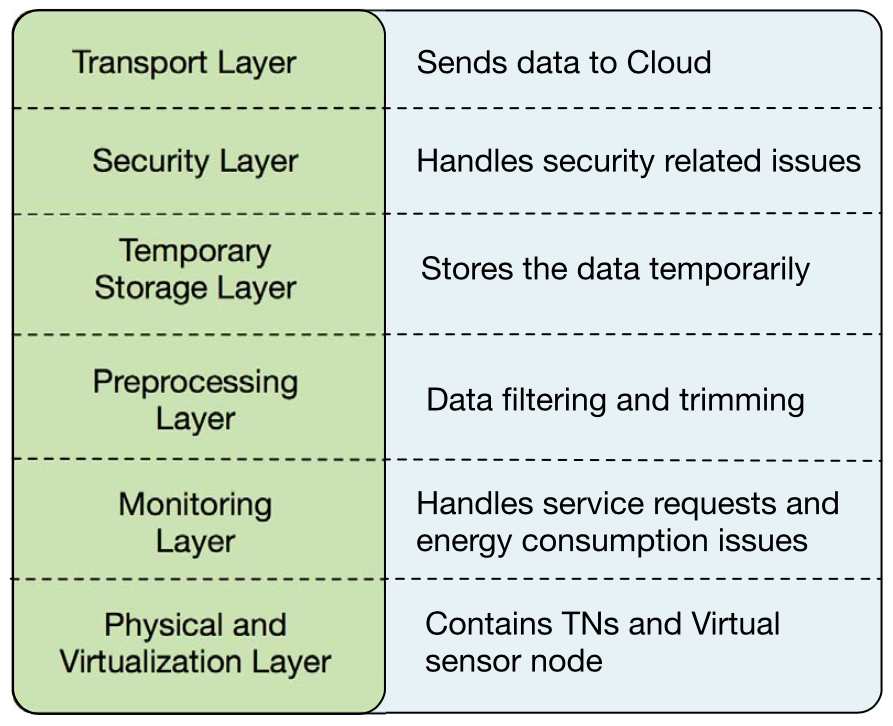
\includegraphics[width=.5\linewidth]{image/Layered architecture for fog computing.png}
    \caption{Layered architecture for fog computing}
    \caption*{img src: \cite{mukherjee2018survey}}
    \label{fig:layered architecture for fog computing}
\end{figure}

The temporary storage layer stores the data temporarily \cite{mukherjee2018survey} as a replica with the help of virtual storage before moving it to the cloud \cite{webpage}. Once the data is sent to the cloud, temporary data stored in this layer will be removed \cite{webpage}. \par

The security layer handles all the issues related to security \cite{mukherjee2018survey}. Ensures privacy, integrity, encryption, and decryption of the data \cite{webpage}. \par

The transport layer sends the data to the cloud \cite{mukherjee2018survey} for permanent storage \cite{webpage}. To achieve efficiency only part of the data is sent to the cloud \cite{webpage}.

%-----------------------------------------------------------------subsection2

\subsection{Networking}

%------------------------------subsubsection2.1

\subsubsection{Fog computing architecture using Software-Defined Networking (SDN)}

Integrated hardware and software are used for conventional networking to direct traffic through a series of routers and switches \cite{yt}. According to \cite{mukherjee2018survey} "Software-Defined Networking (SDN), is an emerging solution that provides a flexible way to update and reconfigure the network." The main idea behind SDN is to virtualize the network \cite{yt} by separating the control plane and the data plane \cite{mukherjee2018survey}. The control plane manages the network and the data plane is where the traffic flows \cite{yt}. OpenFlow is an open protocol between the control plane and data plane \cite{mukherjee2018survey}, that enables the server to tell network switches where to send packets \cite{marg}. The centralized controller called the SDN controller \cite{mukherjee2018survey} manages all the network traffic \cite{yt} and also handles packet forwarding and other networking functionalities \cite{mukherjee2018survey}. The SDN controllers communicate with switches by establishing a TCP connection. The delay between the SDN controller and the switch is a drawback. And the distributed controller might be a solution for this. But, it does increase the number of controllers as there will be one controller per network, which results in a one-hop delay. One solution is the authority switch, which shares the functions of the controller \cite{mukherjee2018survey}. \par

\begin{figure}[H]
    \centering
    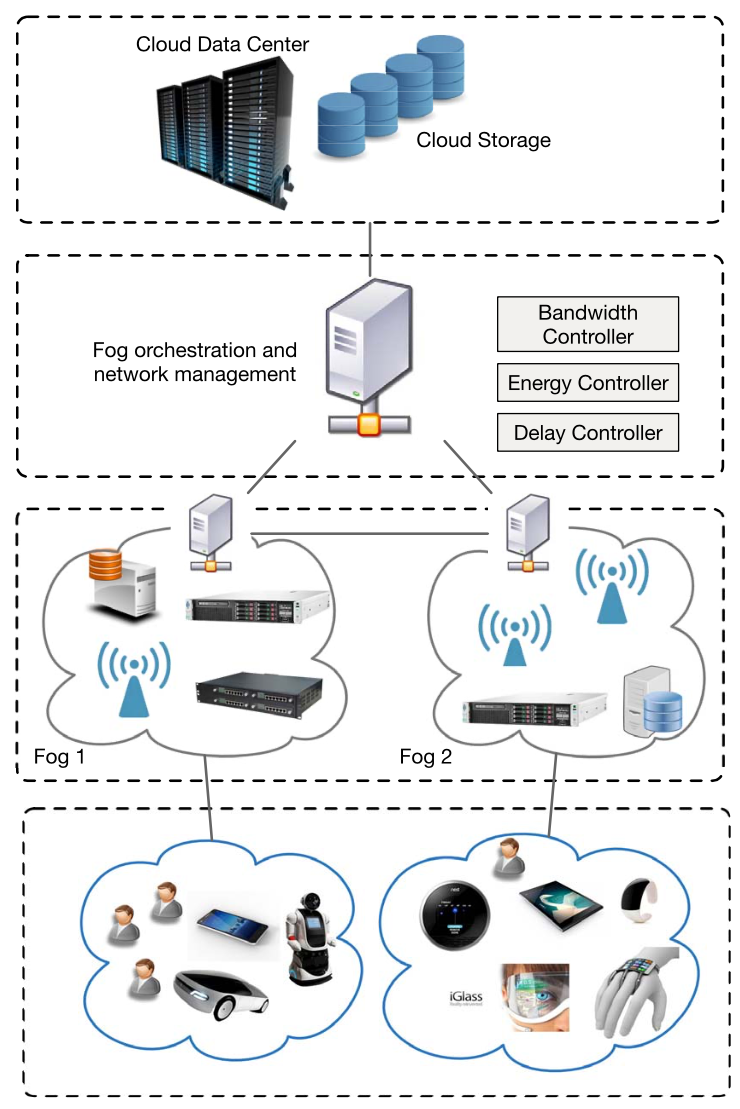
\includegraphics[width=.5\linewidth]{image/SDN-based fog computing architecture.png}
    \caption{SDN-based fog computing architecture}
    \caption*{img src: \cite{mukherjee2018survey}}
    \label{fig:sdn-based fog computing architecture}
\end{figure}

Fog computing is the best approach to provide latency-sensitive services. Even though it is the best option, due to the mobility issues of end devices and traffic distribution, there may be a shortage of available fog computing resources. So, if there are not enough resources in the fog layer, it would be better to transfer some of the latency-aware fog tasks to the cloud. Then, SDN will be aware of the network state and distributes the latency-aware fog tasks. Additionally, dynamic QoS policy deployment is required to handle fog services with different QoS. So, it is important to offer software-defined QoS in fog computing. Therefore, computation and the transmission load on the SDN controller can be minimized. And in SDN-implemented fog networks, scalability and resource management can be improved \cite{mukherjee2018survey}.

Fig. \ref{fig:sdn-based fog computing architecture} shows the SDN-based fog computing architecture. The fog-SDN controller that supports dynamic QoS distinguishes the SDN based architecture from the conventional three-tier architecture of the fog computing. The SDN controller layer defines the QoS based on the attributes and state of the data of the fog node. To get an SDN-based fog computing system, the SDN controller has to support virtualization. To support virtualization, the SDN controller has to be implemented with a hypervisor \cite{mukherjee2018survey}. \par

Fig. \ref{fig:the components of fog-SDN controller} shows the necessary hardware and software components of the fog-SDN controller \cite{mukherjee2018survey}. \par

\begin{figure}[H]
    \centering
    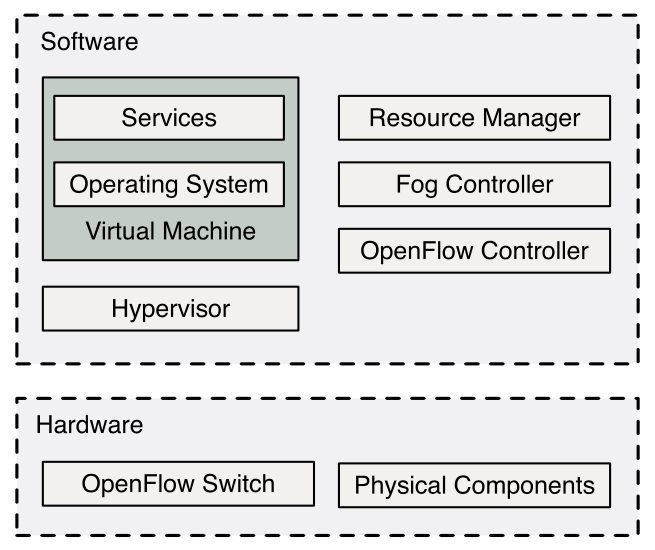
\includegraphics[width=.5\linewidth]{image/The components of fog-SDN controller.png}
    \caption{The components of fog-SDN controller}
    \caption*{img src: \cite{mukherjee2018survey}}
    \label{fig:the components of fog-SDN controller}
\end{figure}

The key concept of SDN is that SDN controllers act as fog orchestration and resource manager \cite{mukherjee2018survey}. \par

According to \cite{sdx} 'SDN orchestration' is "The ability to program automated behaviors in a network to coordinate the required networking hardware and software elements to support applications and services." \par

The fog computing architecture is implemented at edge switches using SDN. It is hard to implement fog computing at switches due to the centralized nature of SDN. So, the controller functionality is integrated at edge switches to perform discrete and distributed computation. Message Queuing Telemetry Transport (MQTT) is used as an IoT protocol for implementation \cite{mukherjee2018survey}.  

Fig. \ref{fig:sdn-based fog (switch) node} shows the framework proposed in \cite{xu2016sdn} to identify and dock/undock applications without EUs interference. The main goal of this framework is to efficiently handle the storage, computation, and networking resources of switches and provide flexibility to SDN by bringing them to the edge of the network. 
The two main components in Fig. \ref{fig:sdn-based fog (switch) node} are Open vSwitch (OvS) and docker management application. The OvS provides a virtual network bridge between individual applications. And it has an SDN controller that handles packet forwarding and other networking functionalities. A virtual Ethernet connection establishes a connection between OvS and docker management application. This framework initiates the flow and manages UEs requests and a pool of applications.

\begin{figure}[H]
    \centering
    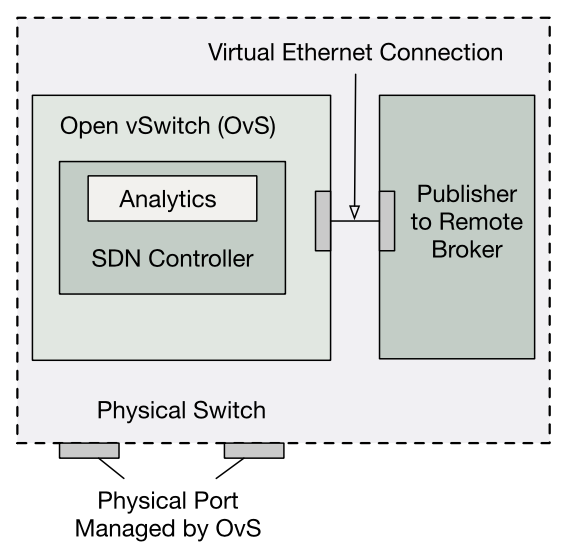
\includegraphics[width=.5\linewidth]{image/SDN-based fog (switch) node.png}
    \caption{SDN-based fog (switch) node}
    \caption*{img src: \cite{mukherjee2018survey}}
    \label{fig:sdn-based fog (switch) node}
\end{figure}

%------------------------------subsubsection2.2

\subsubsection{Fog-Radio Access Networks (F-RANs)}

Radio Access Network (RAN) is a part of cellular technology that establishes a connection between User Equipment (UE) and Core Network (CN) \cite{wi}. It was not easy to manage distributed sites using RAN. So, Cloud-Radio Access Network (C-RAN) was introduced \cite{rf}.  \par 

C-RAN is a centralized architecture for RANs based on cloud computing \cite{mar}. It supports 2G, 3G, 4G \cite{w}, and future wireless communication technologies like 5G and IoT \cite{mar}. C-RAN is also known as Centralized-RAN \cite{w}. The components of C-RAN are Remote Radio Head (RRH), Baseband Unit (BBU) pool, and Mobile Switching Center (MSC). RRH transmits signals, the BBU pool is a central station that processes data, and MSC establishes a connection to the users. Fronthaul connects the BBU pool and RRHs \cite{guizani2017cran}. Backhaul connects the BBU pool to the CN using optical fiber \cite{raj}. \par

Due to the centralized architecture of C-RAN, it is difficult to manage the mobility of users and increased data demand. That increases the burden on fronthaul. To address these issues, Heterogeneous-Cloud Radio Access Network (H-CRAN) which is more efficient than C-RAN was introduced \cite{zhang2017fog}. Instead of the BBU pool, High Power Nodes (HPNs) acts as a central station and does processing in H-CRAN. Fronthaul just transfers the data, and backhaul connects HPNs to the BBU Pools \cite{guizani2017cran}. \par

Fog-Radio Access network (F-RAN) is a hybrid architecture that combines the benefits of H-CRAN and FogNet \cite{mukherjee2018survey}. F-RAN extends resource management, signal processing, distributed storage, and caching capabilities to the edge of the network \cite{zhang2017fog}. The components of F-RAN are Fog-Access Points (F-APs) and Fog-User Equipment (F-UE). F-APs and F-UE do signal processing, have caching capabilities, and Radio Resource Management (RRM) functionalities \cite{guizani2017cran}. Data can be retrieved in this hybrid model in three ways: directly from users, cached at the BBU pool, and from cloud network \cite{mukherjee2018survey}. \par

\begin{figure}[H]
    \centering
    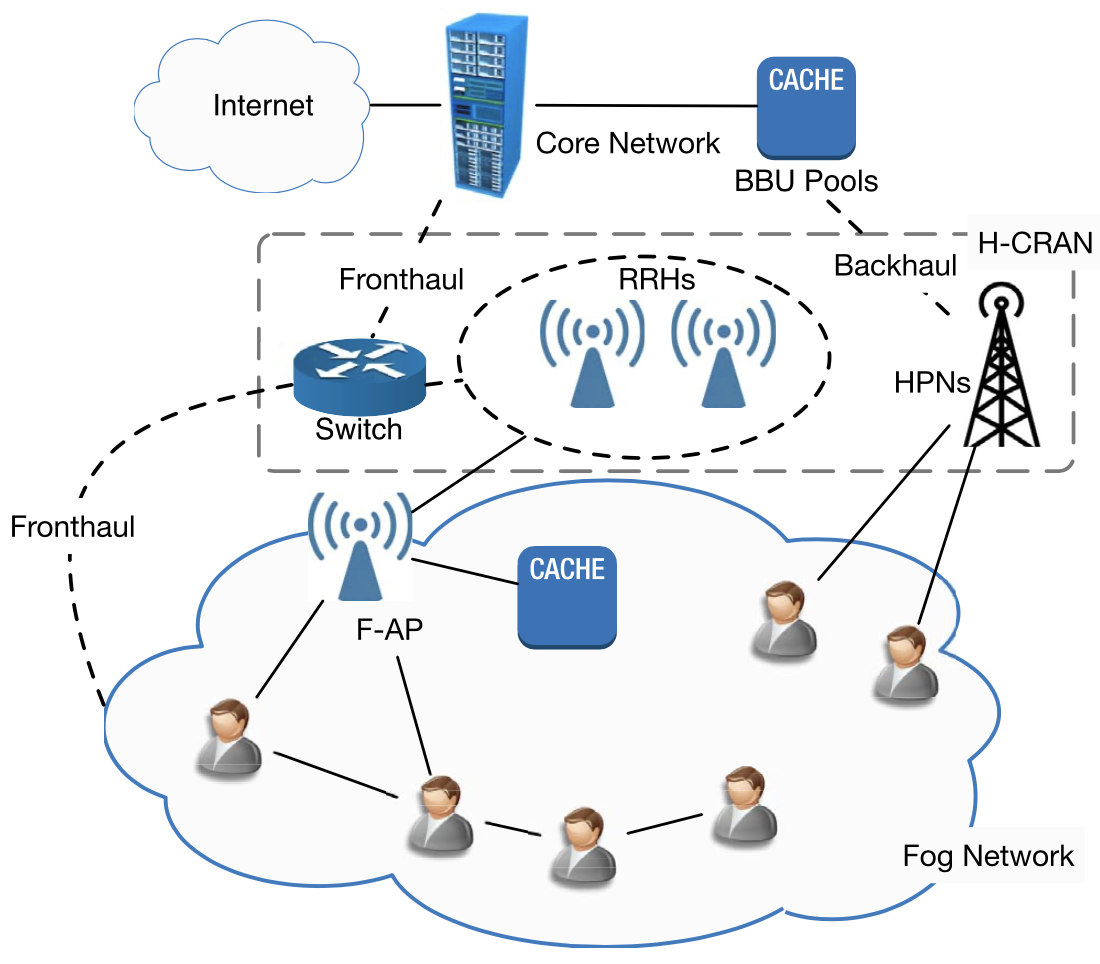
\includegraphics[width=.5\linewidth]{image/FogNet or H-CRAN architecture.png}
    \caption{FogNet/H-CRAN architecture}
    \caption*{img src: \cite{mukherjee2018survey}}
    \label{fig:fognet/h-cran architecture}
\end{figure}

Challenges of F-RAN are \cite{guizani2017cran}:
\begin{itemize}
    \item To support large-scale users and services, the F-RAN requires further research to expand the storage capabilities of both F-APs and F-UEs. Thus, coordinated caching policies for different F-APs and F-UEs need to be ensured \cite{guizani2017cran}.
    \item Implementing SDN is another challenge as an edge network is distributed architecture. Also, the SDN controller is placed in the BBU pool, and fronthaul transfers the data which makes it worse \cite{guizani2017cran}.
\end{itemize}

User access modes:
 \begin{itemize}
    \item D2D mode: D2D mode is selected, when the user requesting the data supports D2D mode, and the requested data is provided by another D2D-enabled user within a predefined distance and the Signal-to-Interference Ratio (SIR) of both the users is greater than the SIR threshold \cite{mukherjee2018survey}.
    \item Nearest F-AP mode: User requesting the data needs access to F-APs if the user does not support D2D mode, and requested data is not available at another D2D-enabled user, and SIR is not greater than threshold \cite{mukherjee2018survey}. 
    \item Local distributed co-ordinated mode: Here, the user requesting the data is connected to multiple F-APs in a user-centric cluster. F-RAN regulates the radius of the cluster to satisfy SIR \cite{mukherjee2018survey}. 
\end{itemize}

%------------------------------subsubsection2.3

\subsubsection{Caching and Offloading}

One of the vital challenges in F-RAN is file caching. Uncoded and coded caching are two caching strategies. The complete file is cached in uncoded caching. But, in coded caching fragments of files are cached in multiple caches using Maximum Distance Separable (MDS) code. RRH caches files until it ran out of memory and processes requests of EUs without using backhaul. But, there will be a burden on backhaul because of the uncached files. So, there should be more number of RRHs for uncached file sharing and less power consumption, and less number of Radio Units (RUs) to reduce the burden on the backhaul. But, due to a lack of cooperation, there will be an increase in power consumption \cite{mukherjee2018survey}. 

\begin{figure}[H]
    \centering
    \includegraphics[width=.5\linewidth]{image/caching policy.png}
    \caption{Caching policy}
    \caption*{img src: \cite{mukherjee2018survey}}
    \label{fig:caching policy}
\end{figure}

In F-RAN, prefetching and delivery are two phases for arbitrary caching. If content popularity is the same, then in prefetching phase processing is done with multiple transmission intervals. But, in the delivery phase on one of the transmission intervals. This depends on data cached during the prefetching phase. Hard and soft-transfer mode are two fronthaul-aware approaches. In hard-transfer mode, data that was not found in the local server was sent from BBU to RRHs. In soft-transfer mode, the quantized version of the baseband signal encoded at BBU is sent to RRHs \cite{mukherjee2018survey}. 